\documentclass[float=false, crop=true]{standalone}
\usepackage{tikz}
\usepackage{xcolor}
\usetikzlibrary{arrows.meta,arrows}
\begin{document}
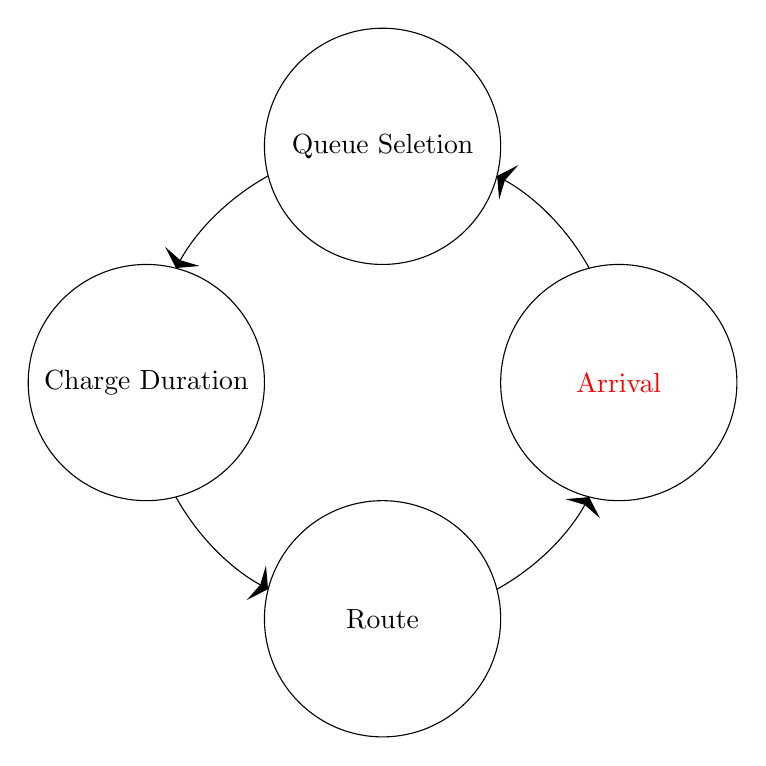
\begin{tikzpicture}

\def \n {4}
\def \radius {3cm}
\def \margin {29} % margin in angles, depends on the radius
\def \text {\textcolor{red}{Arrival}, Queue Seletion, Charge Duration, Route}

\foreach \t [count=\s] in \text
{
  \node[draw, circle, minimum size=3cm] at ({360/\n * (\s - 1)}:\radius) {\t};
  \draw[-{Stealth[width=5mm]}] ({360/\n * (\s - 1)+\margin}:\radius)
    arc ({360/\n * (\s - 1)+\margin}:{360/\n * (\s)-\margin}:\radius);
}
\end{tikzpicture}
\end{document}
